\lhead{\emph{Results}}

This chapter discusses about the results from the experiment with different SMOTE variants. 

10 oversamplers, including Synthsonic, were used in classifying 27 imbalanced datasets shown earlier in table~\ref{tab:df_info}. Due to the large amount of results, it is not feasible to discuss all details of oversampling. For comparison, the average results are shown for all datasets, but also per dataset type. The datasets are separated based on the number of categorical and numerical features in that dataset.

\section{Ranking of oversamplers}
In order to create a fair ranking over all datasets, we have taken the best performance per metric per oversampler. Table~\ref{tab:ranking} overview of the performance over various datasets with different characteristics. The first assumption is that the base classifier without oversampling should perform the worst out of all on most metrics. The exception is precision, which is expected to be higher when there is a high 

\begin{table}[ht]
\centering
    \resizebox{\textwidth}{!}{
    \begin{tabular}{llrlrlrlrlrlr}
    \toprule
    {rank} &        Oversampler &  balanced\_accuracy &        Oversampler &    G\_mean &        Oversampler &        f1 &        Oversampler &  precision &        Oversampler &    recall &        Oversampler &    pr\_auc \\
    \midrule
    1  &             ADASYN &           0.798285 &             ADASYN &  0.729639 &           SVMSMOTE &  0.626186 &     NoOversampling &   0.699163 &             ADASYN &  0.614653 &         synthsonic &  0.649430 \\
    2  &              SMOTE &           0.797884 &              SMOTE &  0.729364 &             ADASYN &  0.623797 &  polynom\_fit\_SMOTE &   0.693186 &         synthsonic &  0.614159 &           SVMSMOTE &  0.649420 \\
    3  &         synthsonic &           0.797308 &         synthsonic &  0.726812 &              SMOTE &  0.621968 &  RandomOversampler &   0.686230 &              SMOTE &  0.614040 &             ADASYN &  0.649238 \\
    4  &           SVMSMOTE &           0.796564 &  RandomOversampler &  0.726309 &       Random\_SMOTE &  0.621696 &           SVMSMOTE &   0.681582 &  RandomOversampler &  0.613770 &  RandomOversampler &  0.648616 \\
    5  &  RandomOversampler &           0.796323 &       Random\_SMOTE &  0.725619 &    BorderlineSMOTE &  0.620457 &       Random\_SMOTE &   0.679765 &       Random\_SMOTE &  0.609360 &  polynom\_fit\_SMOTE &  0.647145 \\
    6  &       Random\_SMOTE &           0.795903 &           SVMSMOTE &  0.724931 &  RandomOversampler &  0.620094 &             ADASYN &   0.678240 &           SVMSMOTE &  0.608782 &              SMOTE &  0.647125 \\
    7  &    BorderlineSMOTE &           0.794202 &    BorderlineSMOTE &  0.724181 &         synthsonic &  0.614133 &    BorderlineSMOTE &   0.675135 &    BorderlineSMOTE &  0.605111 &       Random\_SMOTE &  0.645629 \\
    8  &  polynom\_fit\_SMOTE &           0.781970 &  polynom\_fit\_SMOTE &  0.697985 &  polynom\_fit\_SMOTE &  0.606298 &         synthsonic &   0.671432 &  polynom\_fit\_SMOTE &  0.576800 &    BorderlineSMOTE &  0.642862 \\
    9  &            SMOTENC &           0.768076 &            SMOTENC &  0.693449 &     NoOversampling &  0.580367 &              SMOTE &   0.670155 &            SMOTENC &  0.564887 &     NoOversampling &  0.641915 \\
    10 &     NoOversampling &           0.761715 &     NoOversampling &  0.653643 &            SMOTENC &  0.555265 &            SMOTENC &   0.582476 &     NoOversampling &  0.531739 &            SMOTENC &  0.571079 \\
    \bottomrule
    \end{tabular}}
\caption{A ranking of oversamplers based on their average score of all datasets}
\label{tab:ranking}
\end{table}



\section{Numerical datasets}
The first subcategory of datasets are the ones with either only numerical features or a majority of them. Regular SMOTE techniques are expected to perform better here as their techniques require continuous features to work.

\begin{figure}[htp]
\centering
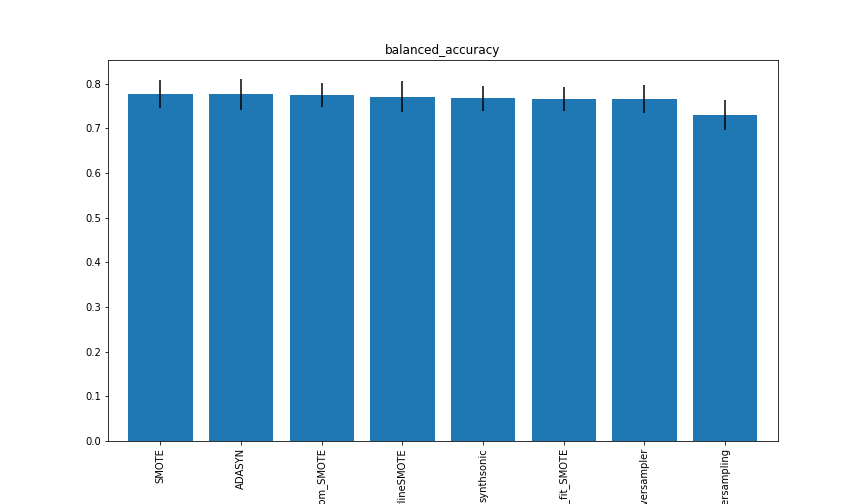
\includegraphics[width=.3\textwidth]{Plots/Plots_numerical_datasets/Numerical_balanced_accuracy.png}\quad
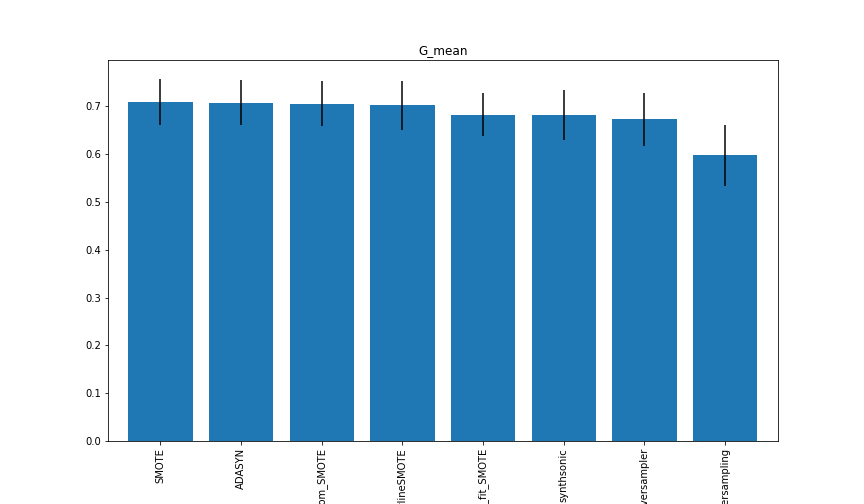
\includegraphics[width=.3\textwidth]{Plots/Plots_numerical_datasets/Numerical_G_mean.png}\quad
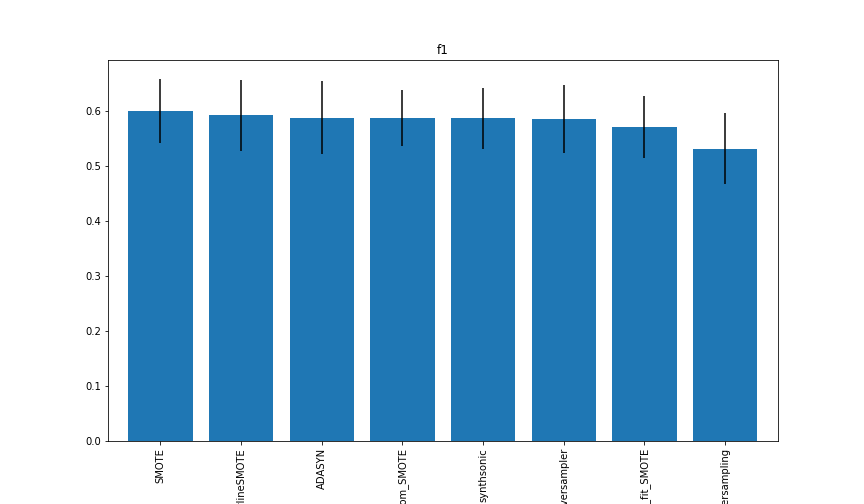
\includegraphics[width=.3\textwidth]{Plots/Plots_numerical_datasets/Numerical_f1.png}

\medskip

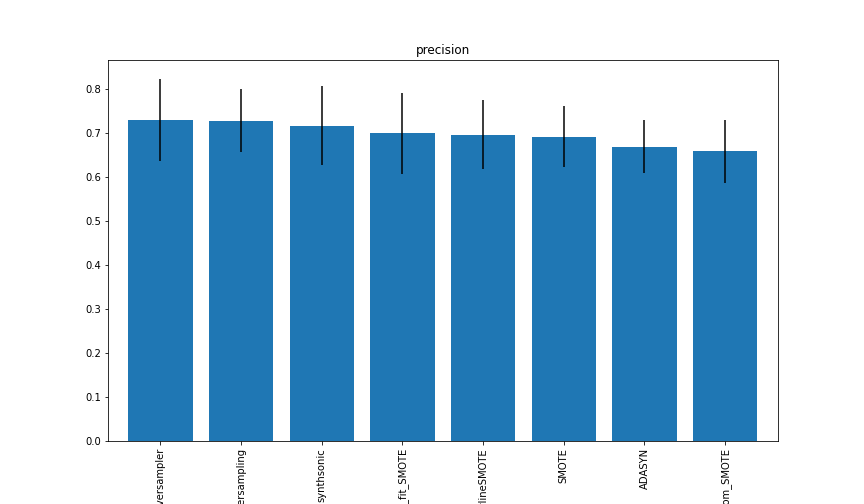
\includegraphics[width=.3\textwidth]{Plots/Plots_numerical_datasets/Numerical_precision.png}\quad
\includegraphics[width=.3\textwidth]{Plots/Plots_numerical_datasets/N}\quad
\includegraphics[width=.3\textwidth]{example-image-b}\quad

\caption{Figure caption}
\label{pics:blablabla}
\end{figure}


\section{Categorical datasets}

\section{Mixed datasets}




